\documentclass[tikz,border=8pt]{standalone}
\usepackage{amsmath,amssymb}
\usetikzlibrary{arrows.meta,calc,decorations.markings,decorations.pathmorphing,patterns,shapes.geometric,positioning}

\begin{document}
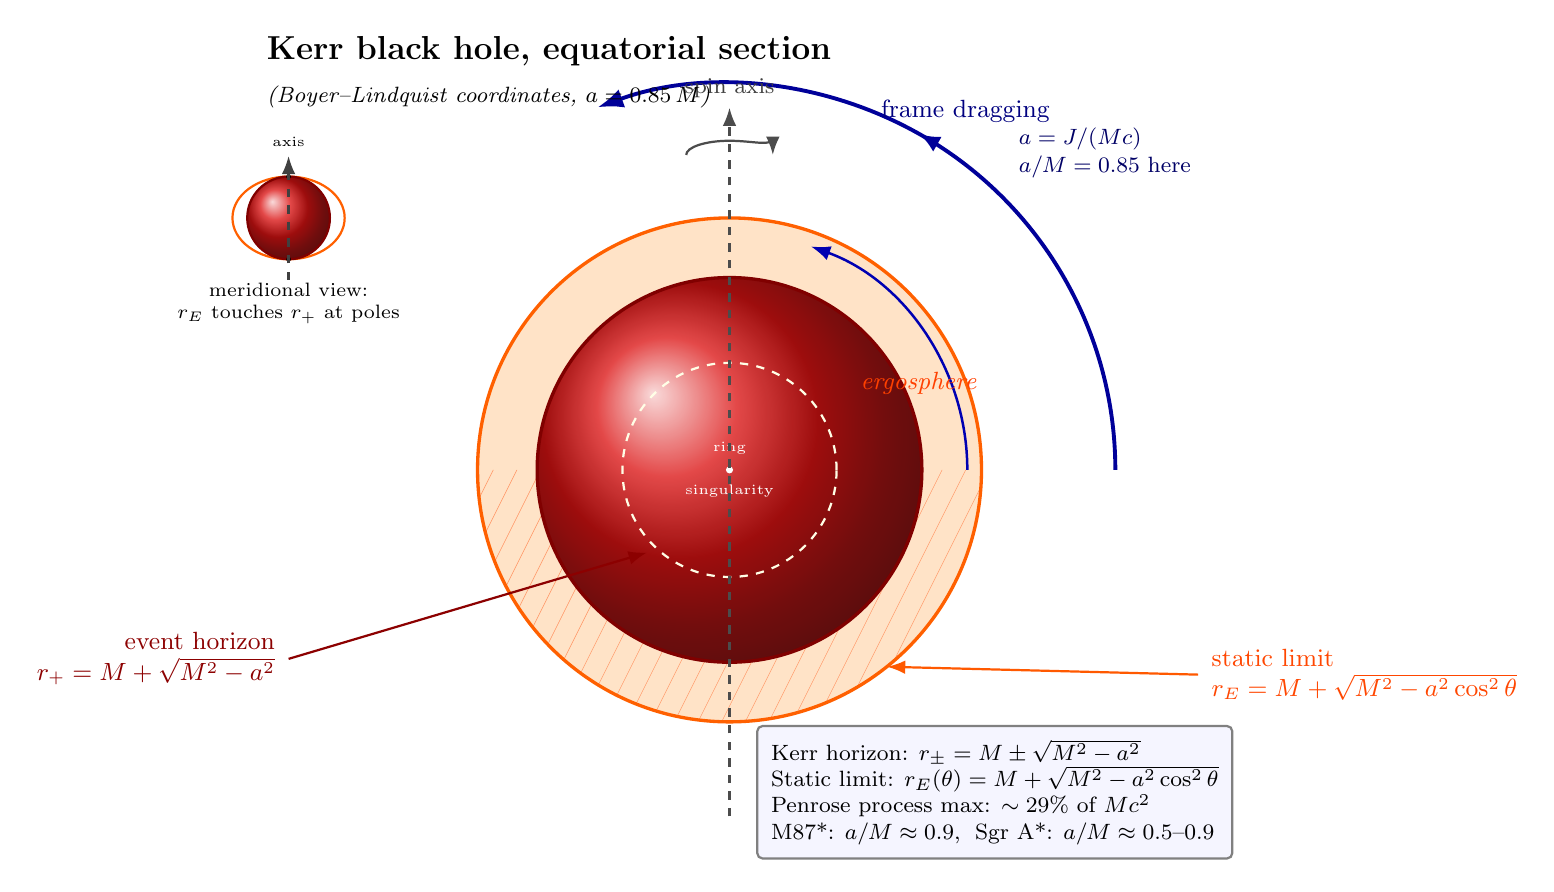
\begin{tikzpicture}[>=Latex]

  % =========================================================================
  % Equatorial cross-section of a Kerr black hole.
  % Use figure units M = 1.0 (geometric units, G=c=1), and choose
  % spin parameter a = 0.85 M for clear visualization.
  %
  %   r_+      = M + sqrt(M^2 - a^2)           (event horizon, sphere)
  %            = 1 + sqrt(1 - 0.7225) = 1 + 0.5267 = 1.527
  %   r_E(eq)  = 2 M = 2.0                      (static limit, equator)
  %   r_E(pol) = M + sqrt(M^2 - a^2)            (static limit, pole = r_+)
  %
  % We draw the equatorial slice. In equatorial section the horizon
  % appears as a circle of radius r_+; the static limit appears as a
  % circle of radius 2M (since cos(theta)=0 in equator). The fact that
  % at the poles r_E meets r_+ is annotated separately (the equatorial
  % view does not show that, so we call it out in a small inset).
  %
  % Scale: 1.6 cm per M unit on canvas.
  % =========================================================================

  \pgfmathsetmacro{\Munit}{1.0}
  \pgfmathsetmacro{\aval}{0.85}
  \pgfmathsetmacro{\rplus}{1.0 + sqrt(1.0 - 0.85*0.85)}      % ~1.527
  \pgfmathsetmacro{\rE}{2.0}                                  % equatorial r_E
  \pgfmathsetmacro{\rRing}{0.85}                              % ring singularity radius = a
  \pgfmathsetmacro{\sc}{1.6}                                  % canvas scale: cm per M

  \pgfmathsetmacro{\Rplus}{\rplus * \sc}                      % ~2.443 cm
  \pgfmathsetmacro{\RE}{\rE * \sc}                            % 3.2 cm
  \pgfmathsetmacro{\RRing}{\rRing * \sc}                      % 1.36 cm

  % --- Background outer halo (faint) ---------------------------------------
  \fill[white] (-6.0, -5.0) rectangle (6.5, 5.5);

  % --- Ergosphere annulus: between r_+ and r_E (orange-yellow shade) -------
  \begin{scope}
    \clip (0,0) circle (\RE);
    \fill[orange!22] (-6,-6) rectangle (6,6);
  \end{scope}
  \begin{scope}
    \clip (0,0) circle (\RE);
    \fill[white] (0,0) circle (\Rplus);
  \end{scope}

  % --- Hatched diagonal pattern in ergosphere for emphasis -----------------
  \begin{scope}
    \clip (0,0) circle (\RE);
    \begin{scope}
      \clip (0,0) circle (\RE);
      \begin{scope}
        % subtract horizon
        \clip (-6,-6) rectangle (6,6) (0,0) circle (\Rplus);
        \foreach \xx in {-6.0,-5.7,...,6.0} {
          \draw[orange!55!red, line width=0.18pt, opacity=0.50]
            (\xx, -6) -- ($(\xx, -6) + (3, 6)$);
        }
      \end{scope}
    \end{scope}
  \end{scope}

  % --- Static limit (r_E) outline (orange) ---------------------------------
  \draw[orange!75!red, very thick] (0,0) circle (\RE);

  % --- Event horizon: filled deep red disk ---------------------------------
  \shade[ball color=red!85!black, opacity=0.95] (0,0) circle (\Rplus);
  \draw[red!50!black, very thick] (0,0) circle (\Rplus);

  % --- Ring singularity: small dashed circle at radius a -------------------
  % In equatorial slice, the ring is a circle of radius a inside r_+.
  \draw[white!90!yellow, dashed, thick] (0,0) circle (\RRing);
  \fill[white] (0,0) circle (0.045);
  \node[font=\tiny, text=white, anchor=south] at (0, 0.07) {ring};
  \node[font=\tiny, text=white, anchor=north] at (0, -0.07) {singularity};

  % --- Frame dragging arrow (curved, blue) ---------------------------------
  \draw[->, blue!60!black, line width=1.4pt,
        decoration={markings,
          mark=at position 0.55 with {\arrow{Latex[length=2.6mm,width=2.2mm]}}},
        postaction={decorate}]
    (4.9, 0) arc[start angle=0, end angle=110, radius=4.9];
  \node[font=\small, text=blue!50!black, anchor=west]
    at (1.8, 4.55) {frame dragging};

  % Second smaller drag arrow inside the ergosphere
  \draw[->, blue!70!black, line width=0.9pt]
    (\RE - 0.18, 0) arc[start angle=0, end angle=70, radius=\RE - 0.18];

  % --- Spin axis indicator (vertical) and arrow ----------------------------
  \draw[->, gray!60!black, thick, dashed] (0, -4.4) -- (0, 4.6);
  \node[font=\footnotesize, text=gray!50!black, anchor=south] at (0, 4.6)
    {spin axis};

  % --- Curved arrow showing rotation direction near axis -------------------
  \draw[->, gray!60!black, thick]
    (-0.55, 4.0) arc[start angle=180, end angle=0, x radius=0.55, y radius=0.18];

  % --- Labels --------------------------------------------------------------
  % r_+ label with line
  \draw[red!55!black, thick, ->] (-5.6, -2.4) -- (-1.05, -1.05);
  \node[anchor=east, font=\small, text=red!55!black, align=right] at (-5.65, -2.4)
    {event horizon\\$r_+ = M + \sqrt{M^2 - a^2}$};

  % r_E label with line
  \draw[orange!70!red, thick, ->] (5.95, -2.6) -- (2.0, -2.5);
  \node[anchor=west, font=\small, text=orange!55!red, align=left] at (6.0, -2.6)
    {static limit\\$r_E = M + \sqrt{M^2 - a^2\cos^2\theta}$};

  % ergosphere label inside
  \node[font=\small\itshape, text=orange!50!red, anchor=center]
    at (2.4, 1.1) {ergosphere};

  % a parameter label
  \node[font=\footnotesize, text=blue!40!black, anchor=west]
    at (3.55, 4.2) {$a = J/(Mc)$};
  \node[font=\footnotesize, text=blue!40!black, anchor=west]
    at (3.55, 3.85) {$a/M = 0.85$ here};

  % --- Pole annotation (small inset diagram top-left) ---------------------
  % Show schematic side view: at the poles, r_E meets r_+ tangentially.
  \begin{scope}[shift={(-5.6, 3.2)}, scale=0.75]
    % Outer ergosphere (oblate)
    \draw[orange!75!red, thick] (0,0) ellipse [x radius=0.95, y radius=0.7];
    % Inner horizon (sphere -> circle)
    \shade[ball color=red!85!black, opacity=0.95] (0,0) circle (0.7);
    \draw[red!50!black, thick] (0,0) circle (0.7);
    % Polar tangency markers
    \fill[black] (0, 0.7) circle (0.04);
    \fill[black] (0, -0.7) circle (0.04);
    \draw[->, gray!50!black, thick, dashed] (0, -1.05) -- (0, 1.05);
    \node[font=\tiny, anchor=south] at (0, 1.05) {axis};
    \node[font=\scriptsize, anchor=south, align=center] at (0, -1.95)
      {meridional view:\\$r_E$ touches $r_+$ at poles};
  \end{scope}

  % --- Numeric reference box (bottom-right) --------------------------------
  \node[draw=black!50, thick, rounded corners=2pt, fill=blue!4,
        inner sep=5pt, anchor=south east, align=left, font=\footnotesize]
    at (6.4, -4.95)
    {Kerr horizon: $r_\pm = M \pm \sqrt{M^2 - a^2}$\\
     Static limit: $r_E(\theta) = M + \sqrt{M^2 - a^2\cos^2\theta}$\\
     Penrose process max: $\sim 29\%$ of $Mc^2$\\
     M87*: $a/M \approx 0.9$, \;Sgr A*: $a/M \approx 0.5$--$0.9$};

  % --- Title (top) ---------------------------------------------------------
  \node[font=\large\bfseries, anchor=south west] at (-6.0, 5.0)
    {Kerr black hole, equatorial section};
  \node[font=\footnotesize\itshape, anchor=north west] at (-6.0, 5.0)
    {(Boyer--Lindquist coordinates, $a = 0.85\,M$)};

\end{tikzpicture}
\end{document}
